%%% Template originaly created by Karol Kozioł (mail@karol-koziol.net) and modified for ShareLaTeX use

\documentclass[a4paper,11pt]{article}

\usepackage[T1]{fontenc}
\usepackage[utf8]{inputenc}
\usepackage{graphicx}
\usepackage{subcaption}
\usepackage{xcolor}
\usepackage{stmaryrd}

% \renewcommand\familydefault{\sfdefault}
% \usepackage{tgheros}
% \usepackage[defaultmono]{droidmono}
\usepackage{mathrsfs}

\usepackage{amsmath,amssymb,amsthm,textcomp}
\usepackage{enumerate}
\usepackage{multicol}
\usepackage{tikz}
\usepackage{hyperref}

\usepackage{geometry}
\geometry{left=25mm,right=25mm,%
bindingoffset=0mm, top=20mm,bottom=20mm}

\usepackage[table]{xcolor} % Para colorear tablas
\usepackage{colortbl}      % Necesario para \cellcolor
\usepackage{array}         % Para centrar texto en columnas

\setlength{\parskip}{1em}
%\linespread{1.3}

\newcommand{\linia}{\rule{\linewidth}{0.5pt}}

% % custom theorems if needed
% \newtheoremstyle{mytheor}
%     {1ex}{1ex}{\normalfont}{0pt}{\scshape}{.}{1ex}
%     {{\thmname{#1 }}{\thmnumber{#2}}{\thmnote{ (#3)}}}
%
% \theoremstyle{mytheor}
% \newtheorem{defi}{Definition}

% my own titles
\makeatletter
\renewcommand{\maketitle}{
\begin{center}
\vspace{2ex}
{\Large \textsc{\@title}}
\vspace{1ex}
\\
\linia\\
\@author \hfill \@date
\vspace{4ex}
\end{center}
}
\makeatother
%%%

% custom footers and headers
\usepackage{fancyhdr}
\pagestyle{fancy}
\lhead{}
\chead{}
\rhead{}
%\lfoot{Lógica Proposicional}
\cfoot{}
%\rfoot{página \thepage}
\renewcommand{\headrulewidth}{0pt}
\renewcommand{\footrulewidth}{0pt}
%

% code listing settings
\usepackage{listings}
\lstset{
    language=Python,
    basicstyle=\ttfamily\small,
    aboveskip={1.0\baselineskip},
    belowskip={1.0\baselineskip},
    columns=fixed,
    extendedchars=true,
    breaklines=true,
    tabsize=4,
    prebreak=\raisebox{0ex}[0ex][0ex]{\ensuremath{\hookleftarrow}},
    frame=lines,
    xleftmargin=2em,
    framexleftmargin=2em,
    showtabs=false,
    showspaces=false,
    showstringspaces=false,
    keywordstyle=\color[rgb]{0.627,0.126,0.941},
    commentstyle=\color[rgb]{0.133,0.545,0.133},
    stringstyle=\color[rgb]{01,0,0},
    numbers=left,
    numberstyle=\small,
    stepnumber=1,
    numbersep=5pt,
    captionpos=t,
    escapeinside={\%*}{*)}
}

%% SET THEORY %%

\usepackage{mathtools}
\usepackage{xparse}
\DeclarePairedDelimiterX\set[2]{\{}{\}}{\,#1 \;\delimsize\vert\; #2\,}

\newcommand{\eqdef}{\stackrel{\text{def}}{=}}

%% local labels in equations %%

\usepackage{xargs}

\makeatletter
  \newcommandx{\Label}[1][1={\arabic{equation}}]%
    {\refstepcounter{equation}(\theequation)~\ltx@label{{#1}} &&}
\makeatother

%% Proof trees %%

\usepackage{fitch}

\usepackage{etoolbox}
\let\bbordermatrix\bordermatrix
\patchcmd{\bbordermatrix}{8.75}{4.75}{}{}
\patchcmd{\bbordermatrix}{\left(}{\left[}{}{}
\patchcmd{\bbordermatrix}{\right)}{\right]}{}{}

%% circled question mark %%

\usepackage{tikz}
\newcommand*\circled[1]{\tikz[baseline=(char.base)]{
            \node[shape=circle,draw,inner sep=.7pt] (char) {\footnotesize #1};}}
\newcommand{\result}{\circled{?}}

%% Venn Diagrams %%

\usepackage{venndiagram}

%% LOGICAL SYMBOLS %%

\newcommand{\liff}{\leftrightarrow}
\DeclarePairedDelimiterX\FORALL[3]{(}{)}{\,\forall #1 : #2 : #3 \,}
\DeclarePairedDelimiterX\EXISTS[3]{(}{)}{\,\exists #1 : #2 : #3 \,}
\DeclarePairedDelimiterX\eval[1]{\llbracket}{\rrbracket}{#1}
\newcommand{\sem}[1]{\eval{#1}^{\model}}
\newcommand{\semv}[2]{\eval{#2}^{\model,#1}}
\newcommand{\model}{\mathfrak{M}}
\newcommand{\interpretation}{\mathscr{I}}
\DeclareMathOperator{\dom}{dom}
\DeclareMathOperator{\fun}{fun}
\DeclareMathOperator{\rel}{rel}

\DeclareRobustCommand{\svdots}{% s for `scaling'
  \vcenter{%
    \offinterlineskip
    \vspace{5pt}
    \hbox{.}
    \vskip0.25\normalbaselineskip
    \hbox{.}
    \vskip0.25\normalbaselineskip
    \hbox{.}%
  }%
}

%% COMPLETE BOX %%
\def\fillbox{\quad[\qquad]\quad}

%% NO INDENT %%

\setlength{\parindent}{0pt}

%%%% LOCALDEFS %%%%

\newcommand{\ambassador}{\mathsf{ambassador}_1}
\newcommand{\person}{\mathsf{person}_1}
\newcommand{\country}{\mathsf{country}_1}
\newcommand{\sentto}{\mathsf{sentto}_2}
\newcommand{\knight}{\mathsf{knight}_1}
\newcommand{\knave}{\mathsf{knave}_1}
\newcommand{\alice}{\mathsf{alice}}
\newcommand{\bob}{\mathsf{bob}}
\newcommand{\tom}{\mathsf{tom}}
\newcommand{\carl}{\mathsf{carl}}

\newcommand{\assig}{\cellcolor{gray!30}1}
\newcommand{\conf}{\cellcolor{yellow!40}1}
\newcommand{\void}{\cellcolor{white}0}

%%%----------%%%----------%%%----------%%%----------%%%

\begin{document}

\title{Modelo de primer parcial}

\author{Lautaro Luna}

\date{}

\maketitle

\vspace*{-1cm}

\section*{Coloreo de Grafos}



\textbf{Pregunta (a) [2 puntos]} \\
Proponga un grafo con al menos 4 (cuatro) nodos, al menos 6 (seis) aristas, y una forma de colorear dicho grafo con una cantidad mínima de colores.

\textbf{Pregunta (b) [3 puntos]} \\
Mostrar formalmente que el grafo propuesto en la pregunta (a) satisface las siguientes restricciones de coloreo:

\begin{description}
  \item[(R1)] El coloreo es entre nodos y colores: \\
  \( \forall n, c:\ \text{coloring2}(n, c) \rightarrow (\text{node1}(n) \land \text{color1}(c)) \)

  \item[(R2)] Todo nodo tiene un único color:
  \begin{enumerate}
    \item[(a)] \( \forall n:\ \text{node1}(n) \rightarrow (\exists c:\ \text{coloring2}(n, c)) \)
    \item[(b)] \( \forall n, c, c':\ (\text{coloring2}(n, c) \land \text{coloring2}(n, c')) \rightarrow \text{eq2}(c, c') \)
  \end{enumerate}
\end{description}

\textbf{Pregunta (c) [2 puntos]} \\
Teniendo en cuenta los predicados \texttt{node1} y \texttt{edge2}, y quizás otros, formalizar las siguientes propiedades:

\begin{description}
  \item[(P1)] Todo nodo es adyacente a un nodo llamado \texttt{proxy}.
  \item[(P2)] Todo nodo puede alcanzar a cualquier otro nodo en 2 pasos.
\end{description}

\textbf{Pregunta (d) [3 puntos]]} \\
Mostrar formalmente si el grafo propuesto en la pregunta (a) satisface, o no satisface, las propiedades formalizadas en la pregunta (c).

\textbf{Pregunta (e) [1 punto]} \\
Sea \( k \) el número mínimo de colores propuesto en la pregunta (a), justificar que el grafo propuesto en esa misma pregunta no puede colorearse con menos colores.

\newpage

\section{Pregunta (a)}

Se propone el siguiente modelo, que consta de 4 nodos y 6 aristas. La mínima cantidad de colores (k) con la que se puede resolver es 2.

\begin{center}
    \begin{minipage}{0.1 \textwidth}
        \centering
        \textbf{$\bigtriangleup$} \\[4pt]
        \rowcolors{1}{}{blue!80!white}
        \begin{tabular}{>{\columncolor{blue!80!white}\color{white}\centering}m{1em}}
            1 \\
            2 \\
            3 \\
            4 \\
            5 \\
            6 \\
        \end{tabular}
    \end{minipage}
    \begin{minipage}{0.2 \textwidth}
        \centering
        \textbf{$node_1$} \\[4pt]
        \begin{tabular}{@{}c@{\hskip 1em}>{\columncolor{blue!80!white}\color{white}}c@{}}
            1 & 1 \\
            2 & 1 \\
            3 & 1 \\
            4 & 1 \\
            5 & 0 \\
            6 & 0 \\
        \end{tabular}
    \end{minipage}
    \begin{minipage}{0.1 \textwidth}
        \centering
        \textbf{$color_1$} \\[4pt]
        \begin{tabular}{@{}c@{\hskip 1em}>{\columncolor{blue!80!white}\color{white}}c@{}}
            1 & 0 \\
            2 & 0 \\
            3 & 0 \\
            4 & 0 \\
            5 & 1 \\
            6 & 1 \\
        \end{tabular}
    \end{minipage}
    \begin{minipage}{0.1 \textwidth}
        \centering
        \textbf{$Constantes$} \\[4pt]
        \begin{tabular}{@{}c@{\hskip 1em}>{\columncolor{blue!80!white}\color{white}}c@{}}
            a     & 1 \\
            proxy & 2 \\
            c     & 3 \\
            d     & 4 \\
            $c_1$ & 5 \\
            $c_2$ & 6 \\
        \end{tabular}
    \end{minipage}

    \begin{minipage}{0.4 \textwidth}
        \centering
        \textbf{$edge_2$} \\[4pt]
        \begin{tabular}{c@{\hskip 1em}*{8}{>{\columncolor{blue!80!white}\color{white}}c}} % Aplica solo a columnas de datos
            % Encabezado (no tiene formato blanco)
            \rowcolor{white}
            \multicolumn{1}{c}{}           &
            \multicolumn{1}{c}{\textbf{1}} &
            \multicolumn{1}{c}{\textbf{2}} &
            \multicolumn{1}{c}{\textbf{3}} &
            \multicolumn{1}{c}{\textbf{4}} &
            \multicolumn{1}{c}{\textbf{5}} &
            \multicolumn{1}{c}{\textbf{6}} &
            \\
            % Cuerpo (tiene fondo azul y texto blanco) 
            1                              & 0 & 1 & 1 & 0 & 0 & 0 \\
            2                              & 1 & 0 & 0 & 1 & 0 & 0 \\
            3                              & 1 & 0 & 0 & 0 & 0 & 0 \\
            4                              & 0 & 1 & 0 & 0 & 0 & 0 \\
            5                              & 0 & 0 & 0 & 0 & 0 & 0 \\
            6                              & 0 & 0 & 0 & 0 & 0 & 0 \\
        \end{tabular}
    \end{minipage}
    \begin{minipage}{0.4 \textwidth}
        \centering
        \textbf{$coloring_2$} \\[4pt]
        \begin{tabular}{c@{\hskip 1em}*{8}{>{\columncolor{blue!80!white}\color{white}}c}} % Aplica solo a columnas de datos
            % Encabezado (no tiene formato blanco)
            \rowcolor{white}
            \multicolumn{1}{c}{}           &
            \multicolumn{1}{c}{\textbf{1}} &
            \multicolumn{1}{c}{\textbf{2}} &
            \multicolumn{1}{c}{\textbf{3}} &
            \multicolumn{1}{c}{\textbf{4}} &
            \multicolumn{1}{c}{\textbf{5}} &
            \multicolumn{1}{c}{\textbf{6}} &
            \\
            % Cuerpo (tiene fondo azul y texto blanco) 
            1                              & 0 & 0 & 0 & 0 & 1 & 0 \\
            2                              & 0 & 0 & 0 & 0 & 0 & 1 \\
            3                              & 0 & 0 & 0 & 0 & 0 & 1 \\
            4                              & 0 & 0 & 0 & 0 & 1 & 0 \\
            5                              & 0 & 0 & 0 & 0 & 0 & 0 \\
            6                              & 0 & 0 & 0 & 0 & 0 & 0 \\
        \end{tabular}
    \end{minipage}
    \begin{minipage}{0.4 \textwidth}
        \centering
        \textbf{$eq_2$} \\[4pt]
        \begin{tabular}{c@{\hskip 1em}*{8}{>{\columncolor{blue!80!white}\color{white}}c}} % Aplica solo a columnas de datos
            % Encabezado (no tiene formato blanco)
            \rowcolor{white}
            \multicolumn{1}{c}{}           &
            \multicolumn{1}{c}{\textbf{1}} &
            \multicolumn{1}{c}{\textbf{2}} &
            \multicolumn{1}{c}{\textbf{3}} &
            \multicolumn{1}{c}{\textbf{4}} &
            \multicolumn{1}{c}{\textbf{5}} &
            \multicolumn{1}{c}{\textbf{6}} &
            \\
            % Cuerpo (tiene fondo azul y texto blanco) 
            1                              & 1 & 0 & 0 & 0 & 0 & 0 \\
            2                              & 0 & 1 & 0 & 0 & 0 & 0 \\
            3                              & 0 & 0 & 1 & 0 & 0 & 0 \\
            4                              & 0 & 0 & 0 & 1 & 0 & 0 \\
            5                              & 0 & 0 & 0 & 0 & 1 & 0 \\
            6                              & 0 & 0 & 0 & 0 & 0 & 1 \\
        \end{tabular}
    \end{minipage}
\end{center}

\begin{center}
    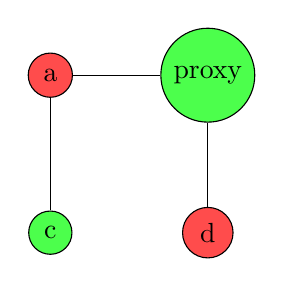
\begin{tikzpicture}
        \node[draw, circle, fill=red!70] (a) at (2,2) {a};
        \node[draw, circle, fill=green!70] (c) at (2,0) {c};
        \node[draw, circle, fill=green!70] (proxy) at (4,2) {proxy};
        \node[draw, circle, fill=red!70] (d) at (4,0) {d};


        \draw (a) -- (proxy);
        \draw (a) -- (c);
        \draw (proxy) -- (d);
    \end{tikzpicture}
\end{center}

\subsection{Formulas a valuar}
\begin{itemize}
    \item $(\forall n, c :: coloring_2(n, c) \Rightarrow (node_1(n) \land color_1(c)))$
    \item $(\forall n :: node_1(n) \Rightarrow (\exists c :: coloring_2(n, c)))$
    \item $(\forall n, c, c' :: coloring_2(n, c) \land coloring_2(n, c') \Rightarrow eq_2(c, c'))$
    \item $(\forall n :: node_1(n) \Rightarrow edge_2(n, 2))$
    \item $(\forall n, m :: node_1(n) \land node_1(m) \Rightarrow (\exists p :: edge_2(n, p) \land edge_2(p, m)))$
    \item $(\exists c :: color_1(c) \Rightarrow (\forall n :: coloring_2(n, c)))$
\end{itemize}

\newpage
\section{Pregunta (b)}
\subsection{R1}

$
    \begin{nd}
        \hypo{}{\eval{(\forall n, c :: coloring_2(n, c) \Rightarrow (node_1(n) \land color_1(c)))}}
        \have{}{min}

        \open
        \hypo{}{\eval{coloring_2(n, c) \Rightarrow node_1(n) \land color_1(c)} \text{ cuando [$n = 1$ y $c \in [1,4] \cup [6]$], o bien}\\
            \text{cuando [$n \in [2,3]$ y $c \in [1,5]$], o bien}\\
            \text{cuando [$n = 4$ y $c \in [1,4] \cup [6]$], o bien}\\
            \text{cuando [$n \in [5,6]$ y $c \in [1,6]$]}}
        \have{}{max(1 - \eval{coloring_2(n, c)}, \eval{node_1(n) \land color_1(c)})}
        \open
        \hypo{}{\eval{coloring_2(n, c)}}
        \have{}{0}
        \close
        \have{}{1}
        \close
        \open
        \hypo{}{\eval{coloring_2(n, c) \Rightarrow node_1(n) \land color_1(c)} \text{ cuando [$n = 1$ y $c = 5$], o bien}\\
            \text{cuando [$n \in [2,3]$ y $c = 6$], o bien}\\
            \text{cuando [$n = 4$ y $c = 5$]}}
        \have{}{max(1 - \eval{coloring_2(n, c)}, \eval{node_1(n) \land color_1(c)})}
        \open
        \hypo{}{\eval{coloring_2(n, c)}}
        \have{}{1}
        \close
        \open
        \hypo{}{\eval{node_1(n) \land color_1(c)}}
        \have{}{min(\eval{node_1(n)}, \eval{color_1(c)})}
        \open
        \hypo{}{\eval{node_1(n)}}
        \have{}{1}

        \close
        \have{}{\eval{color_1(c)}}
        \have{}{1}
        \close

        \have{}{1}
        \close


        \have{}{1}
    \end{nd}
$

\noindent
Esta deducción muestra que {$coloring_2(n, c)$ sólo es verdadera cuando $n$ es un nodo válido y \( c \) un color válido. En todos los casos posibles, la implicación $coloring_2(n, c) \Rightarrow node_1(n) \land color\_1(c)$ se verifica, cumpliendo así con la restricción (R1).

\subsection{R2}
\subsubsection{(a)}
$
    \begin{nd}
        \hypo{}{\eval{(\forall n :: node_1(n) \Rightarrow (\exists c :: coloring_2(n, c)))}}
        \have{}{min}
        \open
        \hypo{}{\eval{node_1(n) \Rightarrow (\exists c :: coloring_2(n, c))} \text{ cuando [$n \in [5] \cup [6]$]}}
        \have{}{max(1 - \eval{node_1(n)},  \eval{\exists c :: coloring_2(n, c)})}
        \open
        \hypo{}{\eval{node_1(n)}}
        \have{}{0}
        \close
        \have{}{1}
        \close

        \open
        \hypo{}{\eval{node_1(n) \Rightarrow (\exists c :: coloring_2(n, c))} \text{ cuando [$n = 1$ y $c = 5$], o bien}\\
            \text{cuando [$n \in [2,3]$ y $c = 6$], o bien}\\
            \text{cuando [$n = 4$ y $c = 5$]}}


        \have{}{max(1 - \eval{node_1(n)},  \eval{\exists c :: coloring_2(n, c)})}
        \open
        \hypo{}{\eval{node_1(n)}}
        \have{}{1}
        \close
        \open
        \hypo{}{\eval{(\exists c ::  coloring_2(n, c)}}
        \have{}{1}
        \close
        \have{}{1}
        \close
        \have{}{1}
    \end{nd}
$

\noindent
Esta deducción verifica que todo nodo válido \( n \) está asociado al menos a un color mediante \( coloring_2(n, c) \). Incluso cuando \( node_1(n) \) es falso, la implicación sigue siendo verdadera por vacuidad. Así, se cumple la restricción (R2a).

\subsubsection{(b)}
$
    \begin{nd}
        \hypo{}{\eval{(\forall n, c, c' :: coloring_2(n, c) \land coloring_2(n, c') \Rightarrow eq_2(c, c'))}}
        \have{}{min}

        \open
        \hypo{}{\eval{coloring_2(n, c) \land coloring_2(n, c') \Rightarrow eq_2(c, c')} \text{ cuando [$n = 1$,  $c \in [1,4] \cup [6]$ y $c' = c $], o bien}\\
            \text{cuando [$n \in [2,3]$, $c \in [1,5]$ y $c' = c$], o bien}\\
            \text{cuando [$n = 4$, $c \in [1,4] \cup [6]$ y $c' = c$], o bien}\\
            \text{cuando [$n \in [5,6]$, $c \in [1,6]$ y $c' = c$]}}
        \have{}{max(1 - \eval{coloring_2(n, c) \land coloring_2(n, c')}, \eval{eq_2(c, c')})}
        \open
        \hypo{}{\eval{coloring_2(n, c) \land coloring_2(n, c')}}
        \have{}{min(\eval{coloring_2(n, c)}, \eval{coloring_2(n, c')})}
        \open
        \hypo{}{\eval{coloring_2(n, c)}}
        \have{}{0}
        \close
        \have{}{0}
        \close
        \have{}{1}
        \close

        \open
        \hypo{}{\eval{coloring_2(n, c) \land coloring_2(n, c') \Rightarrow eq_2(c, c')} \text{ cuando [$n = 1$, $c = 5$, y $c' = c$], o bien}\\
            \text{cuando [$n \in [2,3]$, $c = 6$ y $c' = c$], o bien}\\
            \text{cuando [$n = 4$, $c = 5$ y $c' = c$]}}
        \have{}{max(1 - \eval{coloring_2(n, c) \land coloring_2(n, c')}, \eval{eq_2(c, c')})}
        \open
        \hypo{}{\eval{coloring_2(n, c) \land coloring_2(n, c')}}
        \have{}{min(\eval{coloring_2(n, c)}, \eval{coloring_2(n, c')})}
        \open
        \hypo{}{\eval{coloring_2(n, c)}}
        \have{}{1}

        \close
        \have{}{\eval{coloring_2(n, c')}}
        \have{}{1}
        \close
        \open
        \hypo{}{\eval{eq_2(c, c')}}
        \have{}{1}
        \close


        \have{}{1}
        \close
        \have{}{1}

    \end{nd}
$

\noindent
Esta deducción confirma que si un nodo \( n \) está coloreado con dos colores \( c \) y \( c' \), entonces esos colores deben ser iguales. En todos los casos posibles, \( coloring_2(n, c) \land coloring_2(n, c') \Rightarrow eq_2(c, c') \) se cumple, garantizando que cada nodo tiene un único color asignado, como exige la restricción (R2b).

\section{Pregunta (c)}

\subsection{(P1)}
Todo nodo es adyacente a un nodo llamado proxy. \\
$(\forall n :: node_1(n) \Rightarrow edge_2(n, 2)) \quad \text{(proxy = 2)}$

\subsection{(P2)}
Todo nodo puede alcanzar a cualquier otro nodo en 2 pasos. \\
$(\forall n, m :: node_1(n) \land node_1(m) \Rightarrow (\exists p :: edge_2(n, p) \land edge_2(p, m)))$


\section{Pregunta (d)}

\subsection{(P1)}

$
    \begin{nd}
        \hypo{}{\eval{(\forall n :: node_1(n) \Rightarrow edge_2(n, 2))} \quad \text{(proxy = 2)}}
        \have{}{min}
        \open
        \hypo{}{\eval{node_1(n) \Rightarrow edge_2(n, 2)} \text{ cuando [$n = 3$]}}
        \have{}{max(1 - \eval{node_1(n)}, \eval{edge_2(n, 2)})}
        \open
        \hypo{}{\eval{node_1(n)}}
        \have{}{1}
        \close
        \open
        \hypo{}{\eval{edge_2(n, 2)}}
        \have{}{0}
        \close
        \have{}{0}
        \close
        \have{}{0}

    \end{nd}
$ \\

Esta deducción muestra que la propiedad (P1) no se cumple, ya que existe al menos un nodo válido \( n = 3 \) que no es adyacente al nodo \texttt{proxy} (nodo 2). Por lo tanto, la implicación $(node_1(n) \Rightarrow edge_2(n, 2))$ es falsa para ese caso.

\subsection{(P2)}

$
    \begin{nd}
        \hypo{}{\eval{(\forall n, m :: node_1(n) \land node_1(m) \Rightarrow (\exists p :: edge_2(n, p) \land edge_2(p, m)))}}
        \have{}{min}
        \open
        \hypo{}{\eval{node_1(n) \land node_1(m) \Rightarrow (\exists p :: edge_2(n, p) \land edge_2(p, m))} \text{ cuando [$n = 3$ y $m = 4$]}}
        \have{}{max(1 - \eval{node_1(n) \land node_1(m)}, \eval{(\exists p :: edge_2(n, p) \land edge_2(p, m)})}
        \open
        \hypo{}{\eval{node_1(n) \land node_1(m)}}
        \have{}{min(\eval{node_1(n)}, \eval{node_1(m)})}
        \open
        \hypo{}{\eval{node_1(n)}}
        \have{}{1}
        \close
        \have{}{\eval{node_1(m)}}
        \have{}{1}
        \close
        \open
        \hypo{}{\eval{(\exists p :: edge_2(n, p) \land edge_2(p, m))}}
        \have{}{max}
        \open
        \hypo{}{\eval{edge_2(n, p) \land edge_2(p, m)} \text{ cuando [$p = 1$]}}
        \have{}{min(\eval{edge_2(n, p)}, \eval{edge_2(p, m)})}

        \open
        \hypo{}{\eval{edge_2(n, p)}}
        \have{}{1}
        \close
        \have{}{\eval{edge_2(p, m)}}
        \have{}{0}
        \close

        \open
        \hypo{}{\eval{edge_2(n, p) \land edge_2(p, m)} \text{ cuando [$p \in [2, 6]$]}}
        \have{}{min(\eval{edge_2(n, p)}, \eval{edge_2(p, m)})}
        \open
        \hypo{}{\eval{edge_2(n, p)}}
        \have{}{0}
        \close
        \have{}{0}
        \close

        

        \have{}{0}
        \close

        \have{}{0}

        \close

        \have{}{0}
    \end{nd}
$

\noindent
Esta deducción muestra que la propiedad (P2) no se cumple, ya que existen nodos válidos \( n = 3 \) y \( m = 4 \) para los cuales no se encuentra ningún nodo intermedio \( p \) tal que $edge_2(n, p) \land edge_2(p, m)$. Por lo tanto, no todos los nodos pueden alcanzarse mutuamente en dos pasos.

\section{Pregunta (e)}

$
    \begin{nd}
        \hypo{}{\eval{(\exists c :: color_1(c) \land (\forall n :: coloring_2(n, c)))}}
        \have{}{max}

        \open
        \hypo{}{\eval{color_1(c) \land (\forall n :: coloring_2(n, c)} \text{ cuando [$c \in [1,4] $]}}
        \have{}{min(\eval{color_1(c)}, \eval{(\forall n :: coloring_2(n, c))})}

        \open
        \hypo{}{\eval{color_1(c)}}
        \have{}{0}
        \close
        \have{}{0}
        \close

        \open
        \hypo{}{\eval{color_1(c) \land (\forall n :: coloring_2(n, c)} \text{ cuando [$c = 5$]}}
        \have{}{min(\eval{color_1(c)}, \eval{(\forall n :: coloring_2(n, c))})}

        \open
        \hypo{}{color_1(c)}
        \have{}{1}
        \close

        \open
        \hypo{}{\eval{(\forall n :: coloring_2(n, c))}}
        \have{}{min}
        \open
        \hypo{}{\eval{coloring_2(n, c)} \text{ cuando $n = 2$}}
        \have{}{0}
        \close
        \have{}{0}
        \close      
        \have{}{0}
        \close
        
        \open
        \hypo{}{\eval{color_1(c) \land (\forall n :: coloring_2(n, c)} \text{ cuando [$c = 6$]}}
        \have{}{min(\eval{color_1(c)}, \eval{(\forall n :: coloring_2(n, c))})}

        \open
        \hypo{}{color_1(c)}
        \have{}{1}
        \close

        \open
        \hypo{}{\eval{(\forall n :: coloring_2(n, c))}}
        \have{}{min}
        \open
        \hypo{}{\eval{coloring_2(n, c)} \text{ cuando $n = 1$}}
        \have{}{0}
        \close
        \have{}{0}
        \close      
        \have{}{0}
        \close
        
        \have{}{0}


    \end{nd}
$

\noindent
Esta deducción demuestra que no existe un solo color \( c \) tal que todos los nodos estén coloreados con él. Se evaluaron todos los colores posibles y en ningún caso se cumple \( \forall n:\ coloring_2(n, c) \). Por lo tanto, el grafo no puede colorearse con menos de \( k \) colores, justificando que la cantidad propuesta en la pregunta (a) es mínima.
\end{document}
